\documentclass{beamer}
\usepackage[frenchb]{babel}
\usepackage[T1]{fontenc}
\usepackage[latin1]{inputenc}
\usetheme{Warsaw}
\setbeamercolor{mycolor}{fg=white,bg=black}
\defbeamertemplate*{footline}{shadow theme}{%
\leavevmode%
\hbox{\begin{beamercolorbox}[wd=.5\paperwidth,ht=2.5ex,dp=1.125ex,leftskip=.3cm plus1fil,rightskip=.3cm]{author in head/foot}%
\usebeamerfont{author in head/foot}\hfill\insertshortauthor
\end{beamercolorbox}%
\begin{beamercolorbox}[wd=.4\paperwidth,ht=2.5ex,dp=1.125ex,leftskip=.3cm,rightskip=.3cm plus1fil]{title in head/foot}%
\usebeamerfont{title in head/foot}\insertshorttitle\hfill%
\end{beamercolorbox}%
\begin{beamercolorbox}[wd=.1\paperwidth,ht=2.5ex,dp=1.125ex,leftskip=.3cm,rightskip=.3cm plus1fil]{mycolor}%
\hfill\insertframenumber\,/\,\inserttotalframenumber
\end{beamercolorbox}}%
\vskip0pt%
}
\author{D. Froelicher, A. Marguet, J.Droz, C. Koerckel}
\title{Google Glass}
\date{17 d�cembre 2014}
\begin{document}

\begin{frame}
\titlepage
\begin{figure}
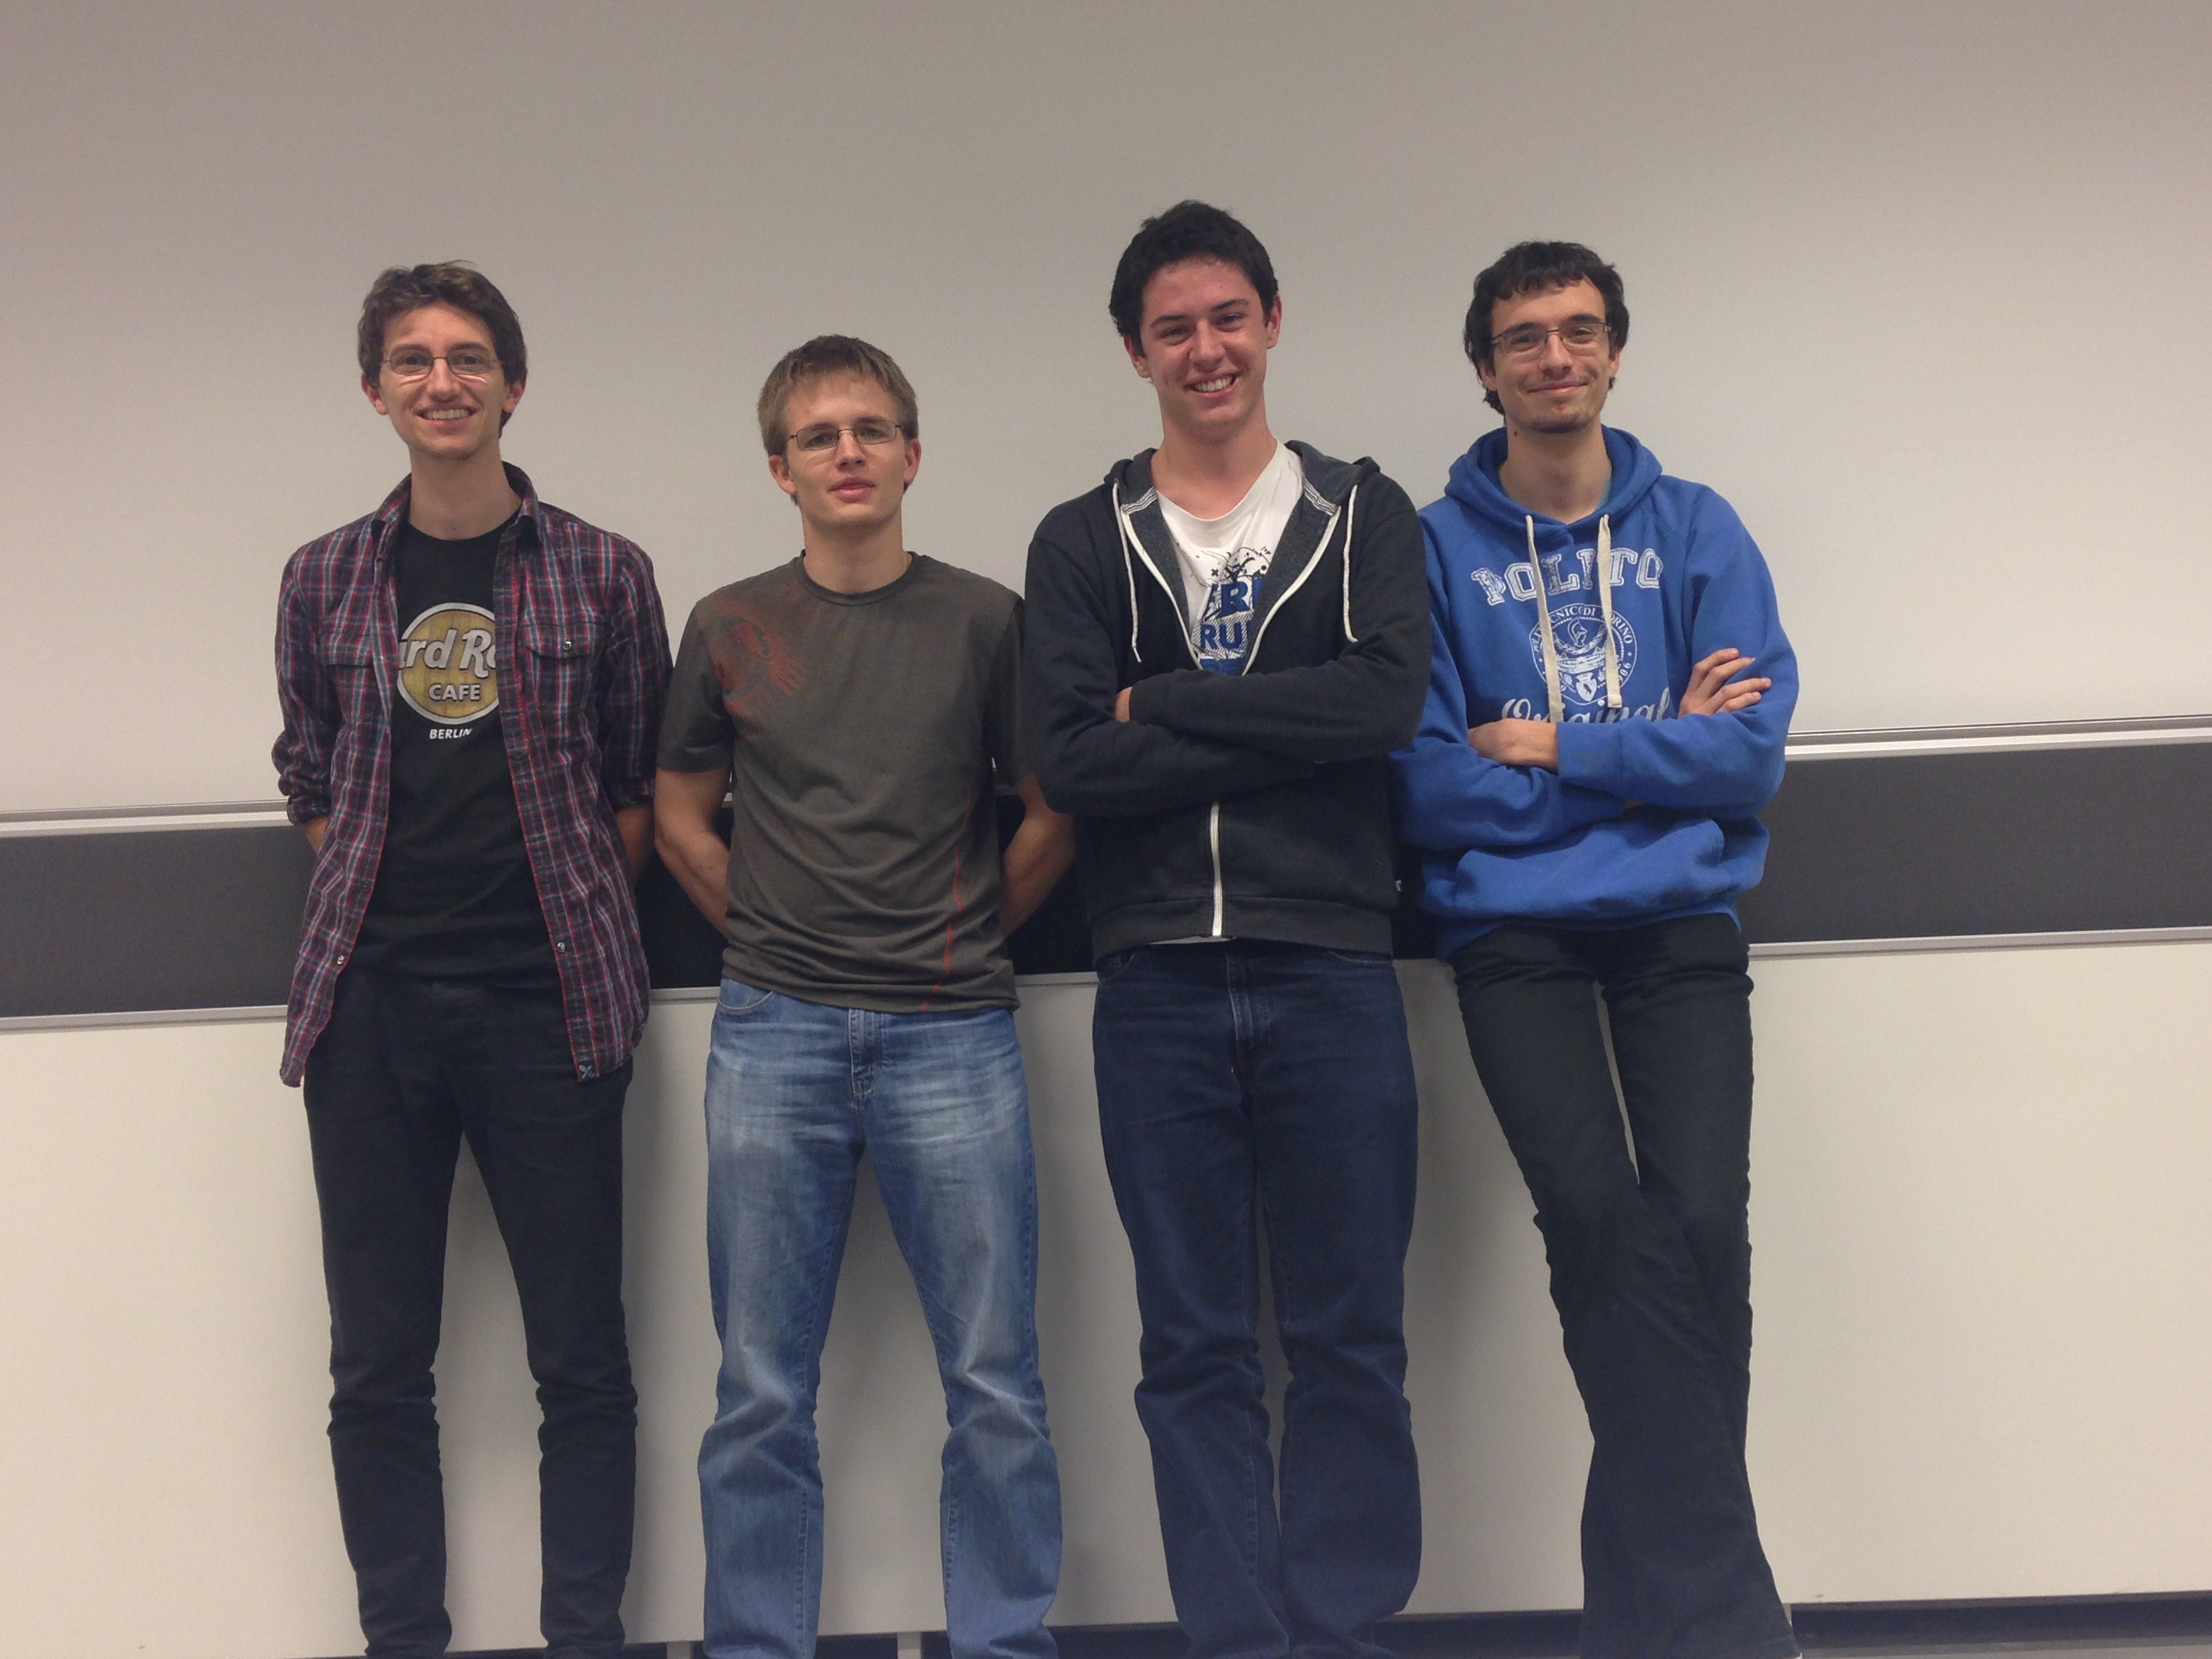
\includegraphics[height=4cm]{portrait.jpg}
\end{figure}
\end{frame}

\begin{frame}
\frametitle{Sommaire}
\tableofcontents
\end{frame}

\begin{frame}
\frametitle{Google Glass}
\begin{figure}
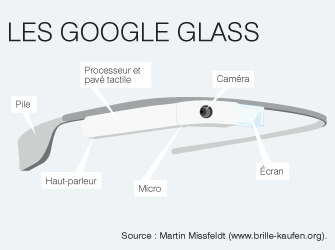
\includegraphics[height=4cm]{glass.jpg}
\end{figure}

\begin{itemize}
\item Cam�ra int�gr�e
\item Micro
\item Pav� tactile
\item Mini �cran
\item Acc�s internet
\item Ecouteur
\end{itemize}
Acc�s � toutes les fonctionnalit�s de google, similaire a un smartphone
\end{frame}


\begin{frame}
\section{Probl�matique}
\frametitle{Probl�matique}
\end{frame}


\begin{frame}
\section{Enjeux soci�taux}
\frametitle{Enjeux soci�taux}
\end{frame}

\begin{frame}
\section{Th�se et hypoth�ses}
\frametitle{Th�se et hypoth�ses}
\end{frame}

\begin{frame}
\section{Motivation personnelles}
\frametitle{Motivation personnelles}
\end{frame}




\end{document}